\section{Лекция номер 12}
\subsection{До перерыва}
gg
\subsection{После перерыва}
Докажем еще пару теорем необходимых для доказательства теоремы об обратной функции.
\begin{theorem}
    Пусть $f: \R^n \to \R^m$ -- функция, дифференерцируемая в шаре $B_r(a)$, и $\forall x \in B_r(a)$ норма $\| f'(x) \| \leqslant C$. 
    Тогда $\forall x, y \in B_r(a)$ выполняется $\| f(x) - f(y) \| \leqslant C \| x - y \|$.
\end{theorem}
\begin{proof}
    Введем $\varphi:[0, 1] \to \R \;\; \varphi(t) = \langle f(x + t(y - x)), f(y) - f(x) \rangle$.
    Она дифференерцируема, так как $f(x + t(y - x))$ дифференерцируема, ведь отрезок $[x, y] \in B_r(a)$, $f(y) - f(x)$ -- константный вектор, и скалярное произведение дифференерцируемо.

    \quad Согласно одномерной теореме Лагранжа: $\varphi(1) - \varphi(0) = \varphi'(\theta)$, где $\theta \in (0, 1)$. 
    Распишем по формуле дифференцирования скалярного произведения: \begin{gather*}
        \begin{split}
            \varphi'(\theta) &= \langle f'(x + \theta(y - x))*(y - x), f(y) - f(x) \rangle + \underbrace{\langle f(x + \theta(y - x)), 0 \rangle}_0  \\
            &\overset{\text{КБШ}}{\leqslant} \| f'(x + \theta(y - x))*(y - x) \| * \| f(y) - f(x) \| \\
            &\leqslant \| f'(x + \theta(y - x))\| * \| y - x \| * \| f(y) - f(x) \| \\
            &\leqslant C\| y - x \| * \| f(y) - f(x) \|
        \end{split}
    \end{gather*}
    \quad Распишем $\varphi(1) - \varphi(0)$ по определению: \begin{gather*}
        \varphi(1) - \varphi(0) = \langle f(y), f(y) - f(x) \rangle - \langle f(x), f(y) - f(x) \rangle = \\
        = \langle f(y), f(y) \rangle - 2 \langle f(y), f(x) \rangle +  \langle f(x), f(x) \rangle = \| f(y) - f(x) \|^2 \\ \\
        \Rightarrow \| f(y) - f(x) \|^2 \leqslant C \| y - x \| * \| f(y) - f(x) \| \\
        \Rightarrow \| f(y) - f(x) \| \leqslant C \| y - x \|
    \end{gather*} 
\end{proof}

\begin{theorem} (об обратимости оператора близкого к обратимому) \\
    Пусть $\A: \R^n \to \R^n$ -- линейный обратимый оператор, $\B: \R^n \to \R^n$ -- просто линейный оператор, и выполняется $\| \B - \A \| \leqslant \frac{1}{\| \A^{-1} \|}$ (они достаточно близки).
    Тогда $\B$ обратим, \\ $\| \B^{-1} \| \leqslant \frac{1}{\frac{1}{\| \A^{-1} \|} - \| \B - \A \|}$ и обратные также достаточно близки $\| \B^{-1} - \A^{-1} \| \leqslant \frac{\| \A^{-1} \| * \| \B - \A \|}{\frac{1}{\| \A^{-1} \|} - \| \B - \A \|}$.
\end{theorem}
\begin{proof}
    Напишем неравенство треугольника: \begin{gather*}
        \| \A x \| = \| (\A - \B)x + \B x \| \leqslant \| (\A - \B)x \| + \| \B x \| \\
        \Rightarrow \| \B x \| \geqslant \| \A x \| - \| (\A - \B)x \|
    \end{gather*}
    \quad Заметим, что по стандартному неравенству $\| (\A - \B)x \| \leqslant \| \A - \B \| \| x \|$, а также $\| \A^{-1}(\A x) \| \leqslant \| \A^{-1} \| \| \A x \| \Rightarrow \| \A x \| \geqslant \frac{\| x \|}{\| \A^{-1} \| }$. 
    Подставим все это в неравенство: \begin{gather*}
        \| \B x \| \geqslant  \frac{\| x \|}{\| \A^{-1} \|} - \| \A - \B \| \| x \| = \underbrace{\left(\frac{1}{\| \A^{-1} \|} - \| \A - \B \| \right)}_{=: m} \| x \|
    \end{gather*}
    \quad Тогда по предпредыдущей тоереме $\B$ обратим и $\| \B^{-1} \| \leqslant \frac{1}{m} = \frac{1}{\frac{1}{\| \A^{-1} \|} - \| \B - \A \|}$. 
    Осталось только неравенство на норму разности: \[ \| \B^{-1} - \A^{-1} \| = \| \B^{-1}(\A - \B)\A^{-1} \| \leqslant \| \B^{-1}\| \| \A - \B \| \| \A^{-1} \| \leqslant \frac{1}{m}\| \A - \B \| \| \A^{-1} \| = \frac{\| \A^{-1} \| * \| \B - \A \|}{\frac{1}{\| \A^{-1} \|} - \| \B - \A \|}  \] 
\end{proof}

Теперь мы готовы сформулировать и доказать главную теорему данного параграфа -- теорему об обратной функции.
Храбров назвал ее самой сложной теоремой курса, так что пристегните ремни.

\underline{Мотивация}

\quad \textit{На данный момент мы знаем условия на то, чтобы линейное отображние было обратимо.
Например, определитель его матрицы не должен быть равен 0. 
Хочется понять, существуют ли такие условия для не линейного, а просто непрерывно дифференерцируемого отображения.
Оказывается, что глобальной обратимости у нас не будет, а вот локальная вполне будет существовать, если отображение будет достаточно хорошим.
Более формально: если у нас в точке дифференциал обратим, то в небольшой окрестности этой точки наше отображение будет вести себя примерно как линейное, а значит будет обратимо.}

\begin{theorem} (об обратной функции) \\
    Пусть
    \begin{itemize}
        \item $f: D \to \R^n$, где $D \subset \R^n$ -- открытое
        \item $x_0 \in D$, причем $f$ непрерывно дифференерцируемо в окр-ти $x_0$; $y_0 = f(x_0)$
        \item линейное отображение $\A = f'(x_0)$ обратимо (дифференциал в точке обратим)
    \end{itemize} 
    Тогда $\exists \, U$ -- окр-ть точки $x_0$, $\exists \, V$ -- окр-ть точки $y_0$, т.ч. $f: U \to V$ обратимо и  $f^{-1}: V \to U$ непрерывно.
\end{theorem}
\begin{proof}
    Введем отображение $G_y(x) := x + \A^{-1}(y - f(x))$.
    Выберем $B_r(x_0)$ так, что $\forall x \in B_r(x_0)$ выполняется $\| \A^{-1} \| * \| \A - f'(x) \| \leqslant \frac{1}{2}$.
    Мы действительно так можем сделать, потому что $\| \A^{-1} \|$ -- это константа, а $f$ непрерывно дифференерцируемо в окр-ти $x_0$, т.е. при $x$ близком к $x_0$ имеем $f'(x)$ близкое к $\A$. 
    Благодаря этому неравенству мы можем применить предыдущую теорему. 
    Получаем, что $f'(x)$ обратимо для $x \in B_r(x_0)$ (честно говоря, я так и не понял, где мы это дальше использовали; если вы это поняли, отредактируйте / напишите кому-то из составителей).

    \quad Теперь мы хотим, чтобы $G_y(x)$ было сжатием. 
    Для этого нам надо понять, что норма ее производной небольшая: \[ \| G_y'(x) \| = \| \underbrace{\mathcal{E}}_{\text{ед. оп.}} + \underbrace{(\A^{-1}(y))'}_{= c' = 0} - \underbrace{(d_{f(x)}\A^{-1} \circ d_xf)}_{\text{опр. диф. комп.}} \| = \| \mathcal{E} - \A^{-1}(f'(x)) \| =\circledast \]
    \quad Мы воспользовались тем, что $d_{f(x)}\A^{-1} = \A^{-1}$. 
    Это так, потому что $\A^{-1}$ -- линейное отображение, следовательно, дифференциал, посчитанный в любой точке, равен ему самому.
    Продолжим оценивать норму производной: \[ \circledast = \| \A^{-1}(\A - f'(x)) \| \leqslant \| \A^{-1} \| * \|(\A - f'(x)) \| \leqslant \frac{1}{2}  \]
    \quad Значит, $G_y$ -- сжатие с коэффициентом $\frac{1}{2}$. 
    
    \quad Заметим, что для того, чтобы эти рассуждения работали, нам необходимо, чтобы $G_y(B_r(x_0)) \subset B_r(x_0)$.
    Действительно, в противном случае при применении $G_y(x)$ мы можем выскочить из шара $B_r(x_0)$, a там уже с $f'(x)$ творится сущий кошмар.

    \quad Подберем $B_R(y_0)$ так, что $\forall y \in B_R(y_0)$ выполняется $G_y(B_r(x_0)) \subset B_r(x_0)$.
    Оценим, как далеко мы отдаляемся при $y \in B_R(y_0)$:
    \begin{gather*}
        \begin{split}
            \| G_y(x) - x_0 \| &\leqslant  \underbrace{\| G_y(x_0) - x_0 \|}_{= x_0 + \A^{-1}(y-f(x_0)) - x_0} + \| G_y(x) - G_y(x_0) \| \\
            &= \| \A^{-1}(y - y_0)\| + \| G_y(x) - G_y(x_0) \| \\
            &\leqslant \| \A^{-1} \| \| y - y_0 \| + \frac{1}{2}\| x - x_0 \| \leqslant R\| \A^{-1} \| + \frac{r}{2}
        \end{split}
    \end{gather*}
    \quad Мы хотим, чтобы $G_y(x)$ попало в шар $B_r(x_0)$. Tаким образом, должно выполняться \\ $\| G_y(x) - x_0 \| < r$.
    С помощью предыдущего неравенства мы легко подберем нужное $R$ и получим необходимый шар $B_R(y_0)$.

    \quad Теперь воспользуемся теоремой Банаха о сжатии. $G_y$ -- это сжимающее отображение, поэтому обязана существовать неподвижная точка:
    \[ \exists \, x \in B_r(x_0) : x = G_y(x) = x + \A^{-1}(y - f(x)) \Rightarrow \A^{-1}(y - f(x)) = 0 \Rightarrow f(x) = y \]
    \quad Заметим, что такой $x$ будет единственнен, так как если $f(x) = y$, то $x$ -- неподвижная точка, а она всего одна.
    Следовательно, у нас нашлась такая окрестность точки $y_0$, что для каждой точки из нее найдется единтсвенный $x$, т.ч. $f(x) = y$.
    Положим $V := B_R(y_0)$ и $U := f^{-1}(V)$ -- открытая окрестность $x_0$.
    Таким образом: $f: U \to V$ -- биекция $\Rightarrow$ существует $f^{-1}: V \to U$.

    \quad Осталось проверить непрерывность $f^{-1}$.
    Пусть $G_y(x) = x$ и $G_{\widetilde{y}}(\widetilde{x}) = \widetilde{x}$.
    Тогда, как мы поняли, $f(x) = y$ и $f(\widetilde{x}) = \widetilde{y}$.
    Нам нужно оценить норму разности обратного отображения: 
    \begin{gather*}
        \| f^{-1}(y) - f^{-1}(\widetilde{y}) \| = \| x - \widetilde{x} \| \underbrace{\leqslant}_{\text{сл. т. Банаха}} \frac{1}{1 - \frac{1}{2}} \| G_y(x) - G_{\widetilde{y}}(x) \| = \\
        = 2 \| x + \A^{-1}(y - f(x)) - x - \A^{-1}(\widetilde{y} - f(x)) \| = 2 \| \A^{-1}(y - \widetilde{y}) \| \leqslant \\
        \leqslant 2 \| \A^{-1} \| \| y - \widetilde{y} \|
    \end{gather*}
    \quad Это и есть критерий непрерывности.
\end{proof}

\vspace*{5mm}

Оказывается, что данное обратное отображение будет не только непрерывным, но и дифференерцируемым.
\begin{theorem} (о дифференерцируемости обратного отображения) \\
    Пусть \begin{itemize}
        \item $f: X \to Y$  -- непрерывное отображение
        \item $f(a) = b$, $U$ -- окр-ть точки $a$, $V$ -- окр-ть точки $b$
        \item $f$ дифференерцируема в точке $a$, $\A = f'(a)$ обратимо
        \item $f^{-1}: V \to U$ существует и непрерывна
    \end{itemize}
    Тогда $g := f^{-1}$ дифференерцируема в точке $b$.
\end{theorem}
\begin{proof}
    Распишем дифференерцируемость в точке $a$: $f(a + h) = f(a) + \A h + \alpha(h)\| h \|$, где $\alpha(h) \to 0$ при $h \to 0$.
    Введем $k := f(a + h) - f(a) = \A h + \alpha(h)\| h \|$. 
    Заведем следующее неравенство: \[ \| h \| = \| \A^{-1}(\A h) \| \leqslant \| \A^{-1} \| \| \A h \| \Rightarrow \| \A h \| \geqslant \frac{\| h \|}{\| \A^{-1} \|} \]
    \quad Используем его при оценке нормы $k$: \[ \| k \| = \| \A h + \alpha(h)\| h \| \| \geqslant \frac{\| h \|}{\| \A^{-1} \|} + \| h \|\|\alpha(h) \| = \| h \| \underbrace{\left(\frac{1}{\| \A^{-1} \|} + \| \alpha(h) \| \right)}_{=:\, C \, > \, 0} \]
    \quad Если $k \to 0$, то $\| h \| \left(\frac{1}{\| \A^{-1} \|} + \| \alpha(h) \| \right) \to 0$, но скобка не будет стремиться к 0, так как $\frac{1}{\| \A^{-1} \|}$ это какая-то константа, поэтому $h \to 0 \text{ т.к. $\alpha(h) \to 0$ }$.
    Вспомним, что $k = f(a+h) - f(a)$, а $g = f^{-1}$. 
    \quad Тогда: \begin{gather*}
        g(\underbrace{b + k}_{f(a+h)}) - g(\underbrace{b}_{f(a)}) = a + h - a = h = \circledast 
    \end{gather*}
    \quad Чтобы выразить $h$ через $k$, применим $\A^{-1}$ к равентсву $k = \A h + \alpha(h)\| h \|$ : \begin{gather*}
        \circledast = \A^{-1}k - \A^{-1}(\alpha(h) \| h \|) \\
        \Rightarrow g(b + k) = g(b) + \A^{-1}k - \A^{-1}(\alpha(h) \| h \|)
    \end{gather*}
    \quad Осталось понять, что $\| \A^{-1}(\alpha(h) \| h \| \| = o(\|k\|)$:
    \[ \| \A^{-1}(\alpha(h) \| h \| \| \leqslant \| \A^{-1} \| * \|\alpha(h) \| * \| h \| \leqslant \| \A^{-1} \| * \underbrace{\|\alpha(h) \|}_{\to 0} * \frac{\|k\|}{C}\  \]
\end{proof}

\begin{follow}
    В теореме об обратной функции $f^{-1}$ непрерывно дифференерцируема в точке $b$.
\end{follow}
\begin{proof}
    Мы поняли, что если обратная функция существует и $f'$ обратима в точке $a$, то обратная функция дифференерцируема в точке $b = f(a)$.
    Это позволяет нам понять, что обратная функция дифференерцируема во всех точках, на которых определена (мы обозначали это множество за $V$).
    Действительно, в док-ве теоремы об обратной функции мы выбирали окр-ть -- $B_r(a)$(там мы использовали $B_r(x_0)$) -- именно так, чтобы $f'$ было там обратимо.
    
    \quad Осталось понять про непрерывность. 
    Введем классическое обозначение матрицы Якоби: $J_f(a)$ -- матрица Якоби $f$ в точке $a$, $J_{f^{-1}}(b)$ -- матрица Якоби $f^{-1}$ в точке $b$.
    Тогда можно применить формулу дифференцирования композиции:
    \begin{gather*}
        f^{-1} \circ f = id \Rightarrow J_{f^{-1} \circ f}(a) = E \\
        J_{f^{-1} \circ f}(a) = J_{f^{-1}}(b) \cdot J_f(a) = E \Rightarrow J_{f^{-1}}(b) = (J_f(a))^{-1} 
    \end{gather*}
    \quad Таким образом, матрица Якоби $f^{-1}$ в точке $b$ -- это обратная к матрице Якоби функции $f$ в точке $a$.
    Мы можем посчитать обратную матрицу с помощью формулы с минорами.
    Тогда мы будем производить разные арифметические операции с частными производными (ведь именно они составляют матрицу Якоби для $f$), а они непрерывны, ведь $f$ непрерывно дифференерцируема по условию.
    В итоге, $J_{f^{-1}}(b)$ будет состоять из различных комбинаций непрерывных функций, то есть частные производные будут непрерывны, а значит  $f^{-1}$ будет непрерывно дифференерцируема в точке $b$.
\end{proof}

\begin{notice}
    Зачастую именно этот вывод называют теоремой об обратной функции.
    Мы же для удобства разбили ее на 3 части.
\end{notice}

\vspace*{7mm}

\begin{follow}
    Пусть $f: \underbrace{D}_{\subset \R^n} \to \R^n$ непрерывно дифференерцируема в $D$ и $f'(x)$ обратимо $\forall x \in D$.
    Тогда для любого открытого $G \subset D$ множество $f(G)$ тоже будет открытым.
\end{follow}

\begin{proof}
    \textit{Fun fact: У нас когда-то было теорема о том, что прообраз открытого мн-ва это всегда открытое мн-во,
    а вот образ открытого это открытое -- явление довольно редкое.} 
    Перейдем к доказательству.

    \quad Зафиксируем произвольное $b \in f(G)$. 
    Надо док-ть, что $b$ -- внутренняя точка. 
    Она лежит в образе $\Rightarrow \exists a : b = f(a)$.
    Применим теорему об обратной функции: $\exists U$ -- окр-ть $a$ и $\exists V$ -- окр-ть $b$, т.ч. $f: U \to V$ -- биекция.
    Заметим, что мы можем выбрать такое $U$, что $U \subset G$. 
    Действительно, надо просто уменьшить нашу окр-ть, чтобы она попала в $G$. 
    Тогда очевидно $f(U) = V \subset f(G)$.
    Получается, что $b \in V \subset f(G)$. 
    Итого, $b$ лежит в $f(G)$ с какой-то окрестностью, следовательно, является внутренней.
\end{proof}

\subsection{ПодводОчка к неявной функции}
\begin{conj}
    Пусть $x \in \R^n, y \in \R^m$. 
    Тогда $(x, y) \in \R^{n + m}$.  
    То есть мы как бы склеиваем их в один большой вектор.
\end{conj}

\begin{notice}
    При применении линейного отображения не надо путать с билинейной формой, т.е. $\A(x, y)$ это применение линейного отображения к одному цельному вектору $(x, y)$.
\end{notice}

\begin{lemma}
    Пусть $\A : \R^{n + m} \to \R^n$ -- линейное отображение, т.ч. $\A(h, 0_m) = 0_n \Rightarrow h = 0_n$.
    \\ Тогда $\forall y \in \R^m$ уравнение $\A(x, y) = 0$ имеет единственное решение.
\end{lemma}
\begin{proof}
    Рассмотрим линейный оператор: \begin{gather*}
        \varphi: \R^n \to \R^n \\
        h \mapsto \A(h, 0)
    \end{gather*}
    \quad Докажем, что $\varphi$ -- биекция.
    Размерности у нас совпадают, поэтому достаточно проверить инъективность.
    Для инъективности же достаточно тривиальности ядра. 
    А это как раз и есть особенность нашего отображения: $\A(h, 0_m) = 0_n \Rightarrow h = 0_n$.

    \quad Вследствие линейности $\A(x, y) = 0 \Leftrightarrow \A(x, 0) = -\A(0, y)$.
    Так как $\varphi$ биекция, мы можем применить обратное отображение:
    \begin{gather*} 
        \varphi^{-1}(\A(x, 0)) = \varphi^{-1}(-\A(0, y)) \\
        x = \varphi^{-1}(-\A(0, y))
    \end{gather*}
    \quad Таким оброазом, при фиксированном $y$ мы однозначно находим $x$. 
\end{proof}

Дальше наша глобальная цель будет состоять в том, чтобы понять, при каком условии уже нелинейные уравнения будут разрешимы.
Но пока что разберем простой пример.

\vspace*{5mm}

\textbf{Пример:}

    \begin{wrapfigure}{r}{6cm} 
        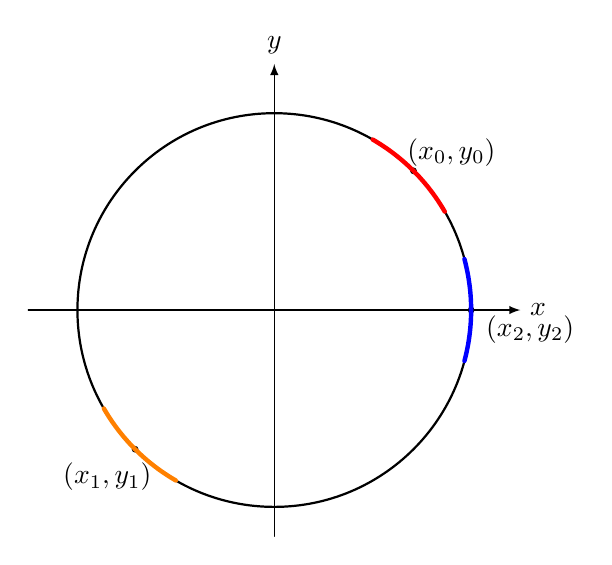
\begin{tikzpicture}[scale=2.5,cap=round,>=latex]
            % draw the coordinates
            \draw[->] (-1.25cm,0cm) -- (1.25cm,0cm) node[right,fill=white] {$x$};
            \draw[->] (0cm,-1.15cm) -- (0cm,1.25cm) node[above,fill=white] {$y$};
    
            % draw the unit circle
            \draw[thick] (0cm,0cm) circle(1cm);
    
            \filldraw[black] (45:1cm) circle(0.4pt)
                            (45:-1cm) circle(0.4pt)
                            (0:1cm) circle(0.4pt);
    
            \draw (1.3cm,-0.1cm) node(b) {$(x_2, y_2)$}
                      (0.9cm,0.8cm) node(a) {$(x_0, y_0)$}
                      (45:-1.2cm) node(c) {$(x_1, y_1)$};
    
            \draw [red,ultra thick,domain=30:60] plot ({cos(\x)}, {sin(\x)});
            \draw [blue,ultra thick,domain=-15:15] plot ({cos(\x)}, {sin(\x)});
            \draw [orange,ultra thick,domain=210:240] plot ({cos(\x)}, {sin(\x)});
    
        \end{tikzpicture}
    \end{wrapfigure}

Рассмотрим уравнение $x^2 + y^2 = 1$.

Если мы изобразим решения этого уравнения, то получится единичная окружность.
Зафиксируем на ней точку $(x_0, y_0)$. 
Если мы будем сдвигаться от нее немного влево и вправо, то у нас получится график функции.

Мы даже можем легко понять, как устроена эта функция: $g(x) = \sqrt{1 - x^2}$.
Так вот такая функция называется неявно заданной уравнением $x^2 + y^2 = 1$.

Если же мы зафиксируем точку $(x_1, y_1)$, то неявная функция примет вид $g(x) = -\sqrt{1 - x^2}$. 
А для точки $(x_2, y_2)$ это уже будет $h(y) = \sqrt{1 - y^2}$. 
Заметим, что для двух предыдущих точек мы также могли записать функцию для $y$.

Теорема о неявной функции как раз и говорит о том, в каком случае мы можем написать неявную функцию для конкретной переменной в конкретной точке.
